\documentclass[11pt,a4paper]{article}
%\pagestyle{headings}
%\linespread{1.6}

% Set up 20 mm margins on each side
\hoffset -5.4mm
\voffset -5.4mm

\oddsidemargin 0.0in
\evensidemargin 0.0in

\textwidth 17.0cm
\textheight 232mm

\topmargin 0.0in
\headheight 4mm
\headsep 9mm
\footskip 12mm

%\usepackage{hyperref,color,graphicx,braket,mathrsfs,simplewick,slashed,amsmath,amssymb,feynmf,ifpdf,pdflscape,wrapfig,fancyhdr,lastpage,etoolbox}
\usepackage{hyperref,xcolor,graphicx,ifpdf,wrapfig,fancyhdr,lastpage,etoolbox,tocloft,multirow,array,pdflscape,enumitem,eurosym,amssymb,titlesec}
\usepackage[square,numbers]{natbib}
%\usepackage[backend=bibtex,style=authoryear]{biblatex}
%\addbibresource{/home/josh/Dropbox/bibliography/xenon_fulbright.bib}

\hypersetup{colorlinks,%
            citecolor=black,%
            linkcolor=black,%
            filecolor=black,%
            urlcolor=black}

\bibliographystyle{JHEP}
%\bibliographystyle{apsrev4-1}

% Set up the header and footer.
\makeatletter
\patchcmd{\@fancyhead}{\rlap}{\color{black}\rlap}{}{}
\patchcmd{\@fancyfoot}{\rlap}{\color{black}\rlap}{}{}
\makeatother

% Set up the title spacing
\titlespacing\section{0pt}{4pt plus 4pt minus 2pt}{0pt plus 2pt minus 2pt}
\titlespacing\subsection{0pt}{4pt plus 4pt minus 2pt}{0pt plus 2pt minus 2pt}
\titlespacing\subsubsection{0pt}{4pt plus 4pt minus 2pt}{0pt plus 2pt minus 2pt}

\pagestyle{fancy}
\fancyhf{}
\renewcommand{\headrulewidth}{0pt}
\lhead{Renner}
\chead{Part B1}
\rhead{DNNEXT}
\cfoot{\thepage}

% To keep the numbering of the table of contents consistent.
\tocloftpagestyle{fancy}

% Table column formatting: from 
% http://tex.stackexchange.com/questions/12703/how-to-create-fixed-width-table-columns-with-text-raggedright-centered-raggedlef
\newcolumntype{L}[1]{>{\raggedright\let\newline\\\arraybackslash\hspace{0pt}}m{#1}}
\newcolumntype{C}[1]{>{\centering\let\newline\\\arraybackslash\hspace{0pt}}m{#1}}
\newcolumntype{R}[1]{>{\raggedleft\let\newline\\\arraybackslash\hspace{0pt}}m{#1}}

\begin{document}
% BB
\newcommand{\bb}{\ensuremath{\beta\beta}}
% BB0NU
\newcommand{\bbonu}{\ensuremath{\beta\beta0\nu}}
% BB2NU
\newcommand{\bbtnu}{\ensuremath{\beta\beta2\nu}}
% NME
\newcommand{\Monu}{\ensuremath{\Big|M_{0\nu}\Big|}}
\newcommand{\Mtnu}{\ensuremath{\Big|M_{2\nu}\Big|}}
% PHASE-SPACE FACTOR
\newcommand{\Gonu}{\ensuremath{G^{0\nu}(\Qbb, Z)}}
\newcommand{\Gtnu}{\ensuremath{G^{2\nu}(\Qbb, Z)}}

% mbb
\newcommand{\mbb}{\ensuremath{m_{\beta\beta}}}
\newcommand{\kgy}{\ensuremath{\rm kg \cdot y}}
\newcommand{\ckky}{\ensuremath{\rm counts/(keV \cdot kg \cdot yr)}}
\newcommand{\mbba}{\ensuremath{m_{\beta\beta}^a}}
\newcommand{\mbbb}{\ensuremath{m_{\beta\beta}^b}}
\newcommand{\mbbt}{\ensuremath{m_{\beta\beta}^t}}
\newcommand{\nbb}{\ensuremath{N_{\beta\beta^{0\nu}}}}

% Qbb
\newcommand{\Qbb}{\ensuremath{Q_{\beta\beta}}}

% Tonu
\newcommand{\Tonu}{\ensuremath{T_{1/2}^{0\nu}}}

% Tonu
\newcommand{\Ttnu}{\ensuremath{T_{1/2}^{2\nu}}}

% Xe-136
\newcommand{\Xe}{\ensuremath{^{136}}Xe}
\newcommand{\COT}{\ensuremath{CO_2}}
\newcommand{\CHF}{\ensuremath{CH_4}}
\newcommand{\CFF}{\ensuremath{CF_4}}

% 2S
\newcommand{\TwoS}{\ensuremath{^{2}S_{1/2}}}

\newcommand{\TwoP}{\ensuremath{^{2}P_{1/2}}}

\newcommand{\TwoD}{\ensuremath{^{2}D_{3/2}}}


% Xe-136
\newcommand{\CS}{\ensuremath{^{137}}Cs}

% Xe-136
\newcommand{\NA}{\ensuremath{^{22}}Na}


% Bi-214
\newcommand{\Bi}{\ensuremath{^{214}}Bi}

% Tl-208
\newcommand{\Tl}{\ensuremath{^{208}}Tl}

% Pb-208
\newcommand{\Pb}{\ensuremath{^{208}}Pb}
% Pb-208
\newcommand{\PBD}{\ensuremath{^{210}}Pb}

% Po-214
\newcommand{\Po}{\ensuremath{^{214}}Po}
\newcommand{\Kr}{\ensuremath{^{83}}Kr}

% bru
\newcommand{\bru}{cts/(keV$\cdot$kg$\cdot$y)}
\newcommand{\dten}{10 mm/$\sqrt{\rm m}$}
\newcommand{\dtwo}{2 mm/$\sqrt{\rm m}$}
\newcommand{\BAPP}{\ensuremath{Ba^{++}}}
\newcommand{\BAP}{\ensuremath{Ba^{+}}}

\newcommand{\HPXE}{\sc{HPXe}\rm}
\newcommand{\BATA}{\sc{BaTa}\rm}

% Saltos de carro en tablas
\newcommand{\minitab}[2][l]{\begin{tabular}{#1}#2\end{tabular}}

\newcommand{\thedraft}{0.1.1}% version for referees

\newcommand{\MO}{\ensuremath{{}^{100}{\rm Mo}}}
\newcommand{\SE}{\ensuremath{{}^{82}{\rm Se}}}
\newcommand{\ZR}{\ensuremath{{}^{96}{\rm Zr}}}
\newcommand{\KR}{\ensuremath{{}^{82}{\rm Kr}}}
\newcommand{\ND}{\ensuremath{{}^{150}{\rm Nd}}}
\newcommand{\XE}{\ensuremath{{}^{136}\rm Xe}}
\newcommand{\GE}{\ensuremath{{}^{76}\rm Ge}}
\newcommand{\GES}{\ensuremath{{}^{68}\rm Ge}}
\newcommand{\TE}{\ensuremath{{}^{128}\rm Te}}
\newcommand{\TEX}{\ensuremath{{}^{130}\rm Te}}
\newcommand{\TL}{\ensuremath{{}^{208}\rm{Tl}}}
\newcommand{\CA}{\ensuremath{{}^{48}\rm Ca}}
\newcommand{\CO}{\ensuremath{{}^{60}\rm Co}}
\newcommand{\PO}{\ensuremath{{}^{214\rm Po}}}
\newcommand{\U}{\ensuremath{{}^{235}\rm U}}
\newcommand{\CT}{\ensuremath{{}^{10}\rm C}}
\newcommand{\BE}{\ensuremath{{}^{11}\rm Be}}
\newcommand{\BO}{\ensuremath{{}^{8}\rm Be}}
\newcommand{\UDTO}{\ensuremath{{}^{238}\rm U}}
\newcommand{\CD}{\ensuremath{^{116}{\rm Cd}}}
\newcommand{\THO}{\ensuremath{{}^{232}{\rm Th}}}
\newcommand{\BI}{\ensuremath{{}^{214}}Bi}


\begin{center}
\large
\textbf{ERC Starting Grant 2017}\\
Research proposal [Part B1]\\[2.0\baselineskip]
\Large
\textbf{Deep Learning in Detector Physics Analyses}\\[1.0\baselineskip]
\LARGE
\textbf{DNNEXT}\\[1.0\baselineskip]
\end{center}
% \vspace{5.5 in}

\noindent PI: Joshua Edward Renner\\
\noindent Host Institution: Universidad de Valencia\\
\noindent Proposal Duration: 60 months\\

The development of deep learning has been realized over the past 10 years with the rise of computing power, which has now permitted the training of neural networks with many layers
of neurons in series.  Such networks have proven capable of high-level abstraction, that is, neurons in deeper layers have been shown to indicate the presence of complex features in a dataset, 
such as the presence of macroscopic objects in images.  It is of great interest to study how such techniques can be applied to physics, and in particular particle detection and tracking, a field 
in which problems exist similar to those to which deep learning has been initially applied.  We propose an in-depth study of the use of deep neural networks in the reconstruction and classification of events in NEXT (Neutrino Experiment with a Xenon TPC), an experiment searching for neutrinoless double beta decay in $^{136}$Xe. We discuss the results that have already been obtained which indicate the advantages of deep neural networks over classical analysis methods and highlight their merit for further study.
\newpage
\normalsize

\newpage
%\setcounter{page}{1}
{\textbf{Section A: Extended Synopsis of the scientific proposal}}

\newpage
\noindent{\textbf{Section B: Curriculum Vitae: Joshua Edward Renner (Postdoctoral Researcher)}}\\[1.0\baselineskip]
\textbf{Renner, Joshua Edward}\\
\textbf{Date of birth:} 30/08/1987\\
\textbf{Nationality:} United States of America\\
\textbf{Email:} jrenner@ific.uv.es\\

%{\noindent\textbf{Research interests}}
%
%\indent\hspace{0.2 cm}\textbullet\,\,Design, analysis, and simulation of particle detectors\\
%\indent\hspace{0.2 cm}\textbullet\,\,Neutrinoless double-beta decay\\
%\indent\hspace{0.2 cm}\textbullet\,\,Deep learning\\

{\noindent\textbf{EDUCATION}}\\

\begin{tabular}{ll}
May 2014 & Ph.D. in Physics\\
& Department of Physics, University of California, Berkeley, CA (U.S.A.)\\
& Advisor: Prof.\ James Siegrist\\

May 2011 & Master of Arts in Physics\\
& Department of Physics, University of California, Berkeley, CA (U.S.A.)\\

May 2009 & Bachelor of Science in Physics\\
& Department of Physics, Georgia Institute of Technology, Atlanta, GA (U.S.A.)\\
\end{tabular}\\

{\noindent\textbf{CURRENT POSITION}}\\

\begin{tabular}{ll}
	July 2016 - & \emph{Investigador Doctor Senior} (Postdoctoral Researcher)\\
	& Instituto de F\'{i}sica Corpuscular (IFIC), University of Valencia, Spain\\
\end{tabular}\\

{\noindent\textbf{PREVIOUS POSITIONS}}\\

\begin{tabular}{ll}
	Sep 2015 - Jun 2016 & \emph{Fulbright Postdoctoral Researcher}\\
	& Instituto de F\'{i}sica Corpuscular (IFIC), University of Valencia, Spain\\
	& and Fulbright Espa\~{n}a\\

	Oct 2014 - Jul 2015 & \emph{Investigador Doctor Junior} (Postdoctoral Research)\\
	& Instituto de F\'{i}sica Corpuscular (IFIC), University of Valencia, Spain\\
	
	May 2009 - May 2014 & \emph{Graduate Student Researcher}\\
	& Lawrence Berkeley National Laboratory (LBNL) and\\
	& University of California, Berkeley, CA (U.S.A.)\\
	& - supported by DOE NNSA SSGF Fellowship Sep 2009 - Aug 2014\\
	& - at Lawrence Livermore National Laboratory May 2010 - Aug 2010\\
	
	May 2007 - Aug 2007, & \emph{Student Employee}\\
	Jan 2008 - Aug 2008 & Georgia Tech Research Institute (GTRI), Atlanta, GA\\
	& Radar Warning Receiver Division\\
\end{tabular}\\

{\noindent\textbf{FELLOWSHIPS}}\\

\begin{tabular}{ll}
	Sep 2015 - Jun 2016 & \emph{Fulbright Junior Research Award}\\
	& Fulbright Espa\~{n}a, Madrid, Spain\\
	& - 9-month research award to continue work on NEXT\\
	
	Sep 2009 - Aug 2014 & \emph{DOE NNSA SSGF Fellowship}\\
	& U.S. Department of Energy (DOE)\\
	& National Nuclear Security Administration (NNSA)\\
	& Stewardship Science Graduate Fellowship (SSGF)\\
	& - 4-year research award covering tuition, fees, and monthly stipend\\
	& - See: http://www.krellinst.org/ssgf\\
	
\end{tabular}\\

\newpage
{\noindent\textbf{TEACHING ACTIVITIES}}\\

\begin{tabular}{ll}
	
	Jul 2016 & \emph{Tutor: IFIC Summer School}\\
	& Instituto de F\'{i}sica Corpuscular (IFIC), University of Valencia, Spain\\
	& - Mentored two undergraduate students during a 2-week summer school\\
	
	Mar 2016 - Apr 2016 & \emph{Tutor: Experimental Project, Masters of Theoretical Physics}\\
	& Instituto de F\'{i}sica Corpuscular (IFIC), University of Valencia, Spain\\
	& - Mentored one Masters student during a 3-week experimental project\\
		
	Aug 2009 - Dec 2009 & \emph{Graduate Student Instructor}\\
	& Dept. of Physics, University of California, Berkeley, CA (U.S.A.)\\
	& - Course: Physics 111, Basic Semiconductor Circuits Laboratory\\
\end{tabular}\\

{\noindent\textbf{WORKSHOPS AND SPECIALIZED SCHOOLS ATTENDED}}\\

\begin{tabular}{ll}
	Sep 4-8, 2013 & \emph{TAUP 2013 Summer School on Astroparticle and Underground Science}\\
	& Asilomar Conference Grounds, Asilomar, CA (U.S.A.)\\
	& - Lecture series\\
	
	Feb 13-24, 2012 & \emph{Excellence in Detectors and Instrumentation Technologies (EDIT) Symposium}\\
	& Fermi National Accelerator Laboratory, Batavia, IL (U.S.A.)\\
	& - Series of lectures and laboratory courses
\end{tabular}\\

\noindent \textbf{PUBLICATIONS AS LEAD AUTHOR AND/OR PRINCIPAL CONTRIBUTOR}\\

\noindent J. Renner, A. Cervera, J. A. Hernando, A. Imzaylov, F. Monrabal, J. Mu\~noz, D. Nygren, and J.J. Gomez-Cadenas.  Improved background rejection in neutrinoless double beta decay experiments using a magnetic field in a high pressure xenon TPC.  JINST 10 (2015) P12020. (arXiv:1509.01821)\\

\noindent J. Renner \emph{et al.} (NEXT Collaboration).  Ionization and scintillation of nuclear recoils in gaseous xenon.  Nucl. Instr. Meth. A 793, 62 (2015).  (arXiv:1409.2853)\\

\noindent V.\ \'{A}lvarez \emph{et al.} (NEXT Collaboration). Near-intrinsic energy resolution for 30 to 662 keV gamma rays in a high pressure xenon electroluminescent TPC. Nucl. Instr. Meth. A 708, 
101 (2013).\\(arXiv:1211.4474)\\
% available online January 18, 2013

\noindent \textbf{SELECTED CONFERENCE PRESENTATIONS}\\

\noindent J. Renner, V. M. Gehman, A. Goldschmidt, D. Nygren, and C.A.B. Oliveira, for the NEXT Collaboration. 
Characterization of Nuclear Recoils in High Pressure Xenon Gas: Towards a Simultaneous Search for WIMP Dark Matter and Neutrinoless 
Double Beta Decay.  TAUP 2013 (presentation by J. Renner on Sept. 11, 2013). Phys. Procedia 61, 766 (2015).\\

\noindent Nuclear Recoils and Recombination in High Pressure Xenon Gas.  Advances in Neutrino Technologies (ANT) 2013 
(presentation by J. Renner on May 11, 2013).\\

\noindent A. Goldschmidt, T. Miller, D. Nygren, J. Renner, D. Shuman, H. Spieler, and J. White.
High-pressure xenon gas TPC for neutrino-less double-beta decay in 136Xe: Progress toward the goal of 1\% FWHM energy resolution.” 
2011 IEEE Nuclear Science Symposium (presentation by J. Renner on Oct. 26, 2011).\\

%{\noindent\textbf{MAJOR COLLABORATIONS}}\\
%
%\indent\hspace{0.2 cm}\textbullet\,\,Assisted in construction and operation of LBNL prototype detector\\
%\indent\hspace{0.2 cm}\,\,\,\,\,\,\,- Primary author of automated data readout and analysis code\\
%\indent\hspace{0.2 cm}\,\,\,\,\,\,\,- Worked on detector electronics and gas system, and PMT calibration\\
%\indent\hspace{0.2 cm}\textbullet\,\,Assisted in mentoring undergraduate students working in the LBNL group\\
%\indent\hspace{0.2 cm}\textbullet\,\,Played a key role in demonstrating 1\% FWHM energy resolution at 662 keV for electrons\\
%\indent\hspace{0.2 cm}\,\,\,\,\,\,\,\,in high pressure xenon gas\\
%\indent\hspace{0.2 cm}\textbullet\,\,Assisted in development of detector Monte Carlo and its execution in supercomputing\\
%\indent\hspace{0.2 cm}\,\,\,\,\,\,\,\,environment\\
%\indent\hspace{0.2 cm}\textbullet\,\,Measured ionization and scintillation produced by nuclear recoils in high pressure xenon\\
%\indent\hspace{0.2 cm}\,\,\,\,\,\,\,\,gas\\
%\indent\hspace{0.2 cm}\textbullet\,\,Developed algorithms to improve background rejection based on event topology\\

\newpage
{\textbf{\emph{Appendix: All on-going and submitted grants and funding of the PI (Funding ID)}}}\\

\noindent\textbf{On-going grants}\\

\noindent\textbf{Grant applications}\\

\newpage
{\textbf{Section C: Early achievements track-record}}

\newpage
\chead{Part B2}
\begin{center}
	\large
	\textbf{ERC Starting Grant 2017}\\
	Research proposal [Part B1]\\[2.0\baselineskip]
\end{center}

\noindent\textbf{Part B2: \underline{The scientific proposal}}\\

{\noindent\textbf{Section A: State-of-the-art and objectives}}\\
In recent years, increasingly sensitive null results (cite) in searches for neutrinoless double beta ($0\nu\beta\beta$) decay have made it clear that an ultra-low background experiment 
employing on the order of tonnes of active mass will be necessary to have a meaningful chance of discovery.  Such an experiment would require excellent energy resolution as well as the use
additional mechanisms for background rejection.  Gaseous xenon enriched in the isotope $^{136}$Xe has shown strong potential for being the 
detection medium of choice for a discovery experiment due to its relatively low cost, ability to act as both source and detector, outstanding energy resolution, and the long ionization 
tracks produced by electrons at energies of order $Q_{\beta\beta}$, which can be analyzed to provide increased background rejection.  NEXT is working towards a presently competitive search 
for $0\nu\beta\beta$ decay with 100 kg of xenon enriched to 90\% in $^{136}$Xe, which will also demonstrate the capacity to benefit from these advantages of gaseous xenon with a 
large detector and thus their potential applicability at the tonne-scale.

Because the senstivity of a background-free $0\nu\beta\beta$ search grows as the square root of the product of the (active mass) $\times$ (exposure time), while in the presence of background the sensitivity increases only as the \emph{fourth} root of the same product, background rejection is of utmost importance. As experiments grow to larger masses, the ability to interpret the information available to reject the maximum amount of background possible becomes vital to the success of the experiment.  It has been recently shown (cite DNN paper) that the conventional analysis of NEXT that has been developed up to this point can be potentially improved using deep neural networks (DNNs) to analyze receonstructed tracks in the experiment. \emph{Such improvements in the analysis will be critical in reaching the ultimate sensitivity of NEXT and in reaching the targeted sensitivity in a larger, tonne-scale experiment.}\\

\noindent\textbf{\textbullet\,\,Objectives}\\
The main objectives of this proposal include:

\begin{enumerate}[itemsep=-1mm]
	\item[1.] To understand the workings and limitations of DNNs as applied to classification and reconstruction in NEXT.
	\item[2.] To produce a DNN-based analysis for NEXT, to be developed and tested alongside acquisition of NEW data.
	\item[3.] To apply the DNN-based analysis to data acquired from the NEXT-100 detector.
	\item[4.] To explore further applications of DNNs in NEXT and particle physics.
\end{enumerate}

\noindent\textbf{Neutrinoless Double-Beta Decay and NEXT}\\
The prospect of demonstrating the Majorana nature of the neutrino and violation of lepton number conservation has inspired a variety of experiments to search for $0\nu\beta\beta$ decay in several candidate isotopes.  The experiments GERDA and EXO, using isotopes $^{76}$Ge and $^{136}$Xe respectively, have set lower limits on the half-life of $0\nu\beta\beta$ decay, $T_{1/2}^{0\nu}$, of greater than $10^{25}$ years.  These and other experiments, such as CUORE, MAJORANA, NEXT, SNO+, and Super-NEMO intend to constrain $T_{1/2}^{0\nu}$ with a lower bound of order $10^{26}$ years.  Recently, KamLAND-ZEN obtained a lower limit of $T_{1/2}^{0\nu} > 1.07\times 10^{26}$ years \cite{KamLANDZen_2016}. The predicted background rate in NEXT-100 is $4 \times 10^{-4}$ counts/(keV kg yr), giving rise to a lower limit on  of $T_{1/2} > 6.0\times 10^{25}$ years (90\% CL) for 3 effective years of running time \cite{NEXT_sensitivity}.  Improvements in background rejection are essential to the operation of NEXT and for realizing sensitivities of order $10^{27}$ years in future tonne-scale experiments.

The core idea behind the NEXT experiment is the electroluminescent (EL) time projection chamber (TPC). In this type of detector, energy is deposited in some active volume filled with a detector medium (high pressure xenon gas, in the case of NEXT), by ionizing radiation such as energetic electrons produced by radioactive decay within the volume or gamma rays which convert via Compton scattering, pair production, or photoabsorption. The ionizing energetic particle produces a track of ionization and excitation in the active medium. The excitation gives rise to scintillation which is detected immediately by photosensors such as photomultiplier tubes (PMTs). This scintillation, called S1, is used to mark the start of the event, after which some delay occurs while the ionized electrons are drifted in an applied electric field to a readout plane at one end of the detector. 

At the readout plane, the ionized electrons are drifted in a much higher electric field through an amplification region in which they are accelerated enough to excite but not ionize the xenon medium.  Each electron produces a number of xenon excitations determined by the magnitude of the electric field in the amplification region, its width, and the operating gas pressure.  These excitations give rise to additional photons (called S2), so that some number of photons is generated for each electron.  The S2 photons generated in this process, called electroluminescence, can then be detected by photosensors to give energy and position information of the event. In NEXT, a cylindrical TPC design is employed, in which a \emph{tracking plane} of silicon photomultipliers (SiPMs) is placed just behind a narrow amplification region, and an \emph{energy plane} of PMTs is installed on one end of the vessel (see figure \ref{fig.SS}, left). In addition to a precise energy measurement to reject background events with energy outside of a narrow region near $Q_{\beta\beta}$, a primary advantage of the NEXT concept is the ability to accurately reconstruct tracks and utilize the topological signature of events to distinguish between signal ($0\nu\beta\beta$) and background events, the majority of which would be produced by gamma rays generating single-electrons.  As also shown in figure \ref{fig.SS}, because of the Bragg peak in energy loss of an energetic electron which gives rise to a dense region (``blob'') of ionization at the end of its ionization track, a two-electron signal event will leave an ionization track with two such ``blobs,'' while a single-electron background event will exhibit only one.

\begin{figure}[!htb]
	\centering
	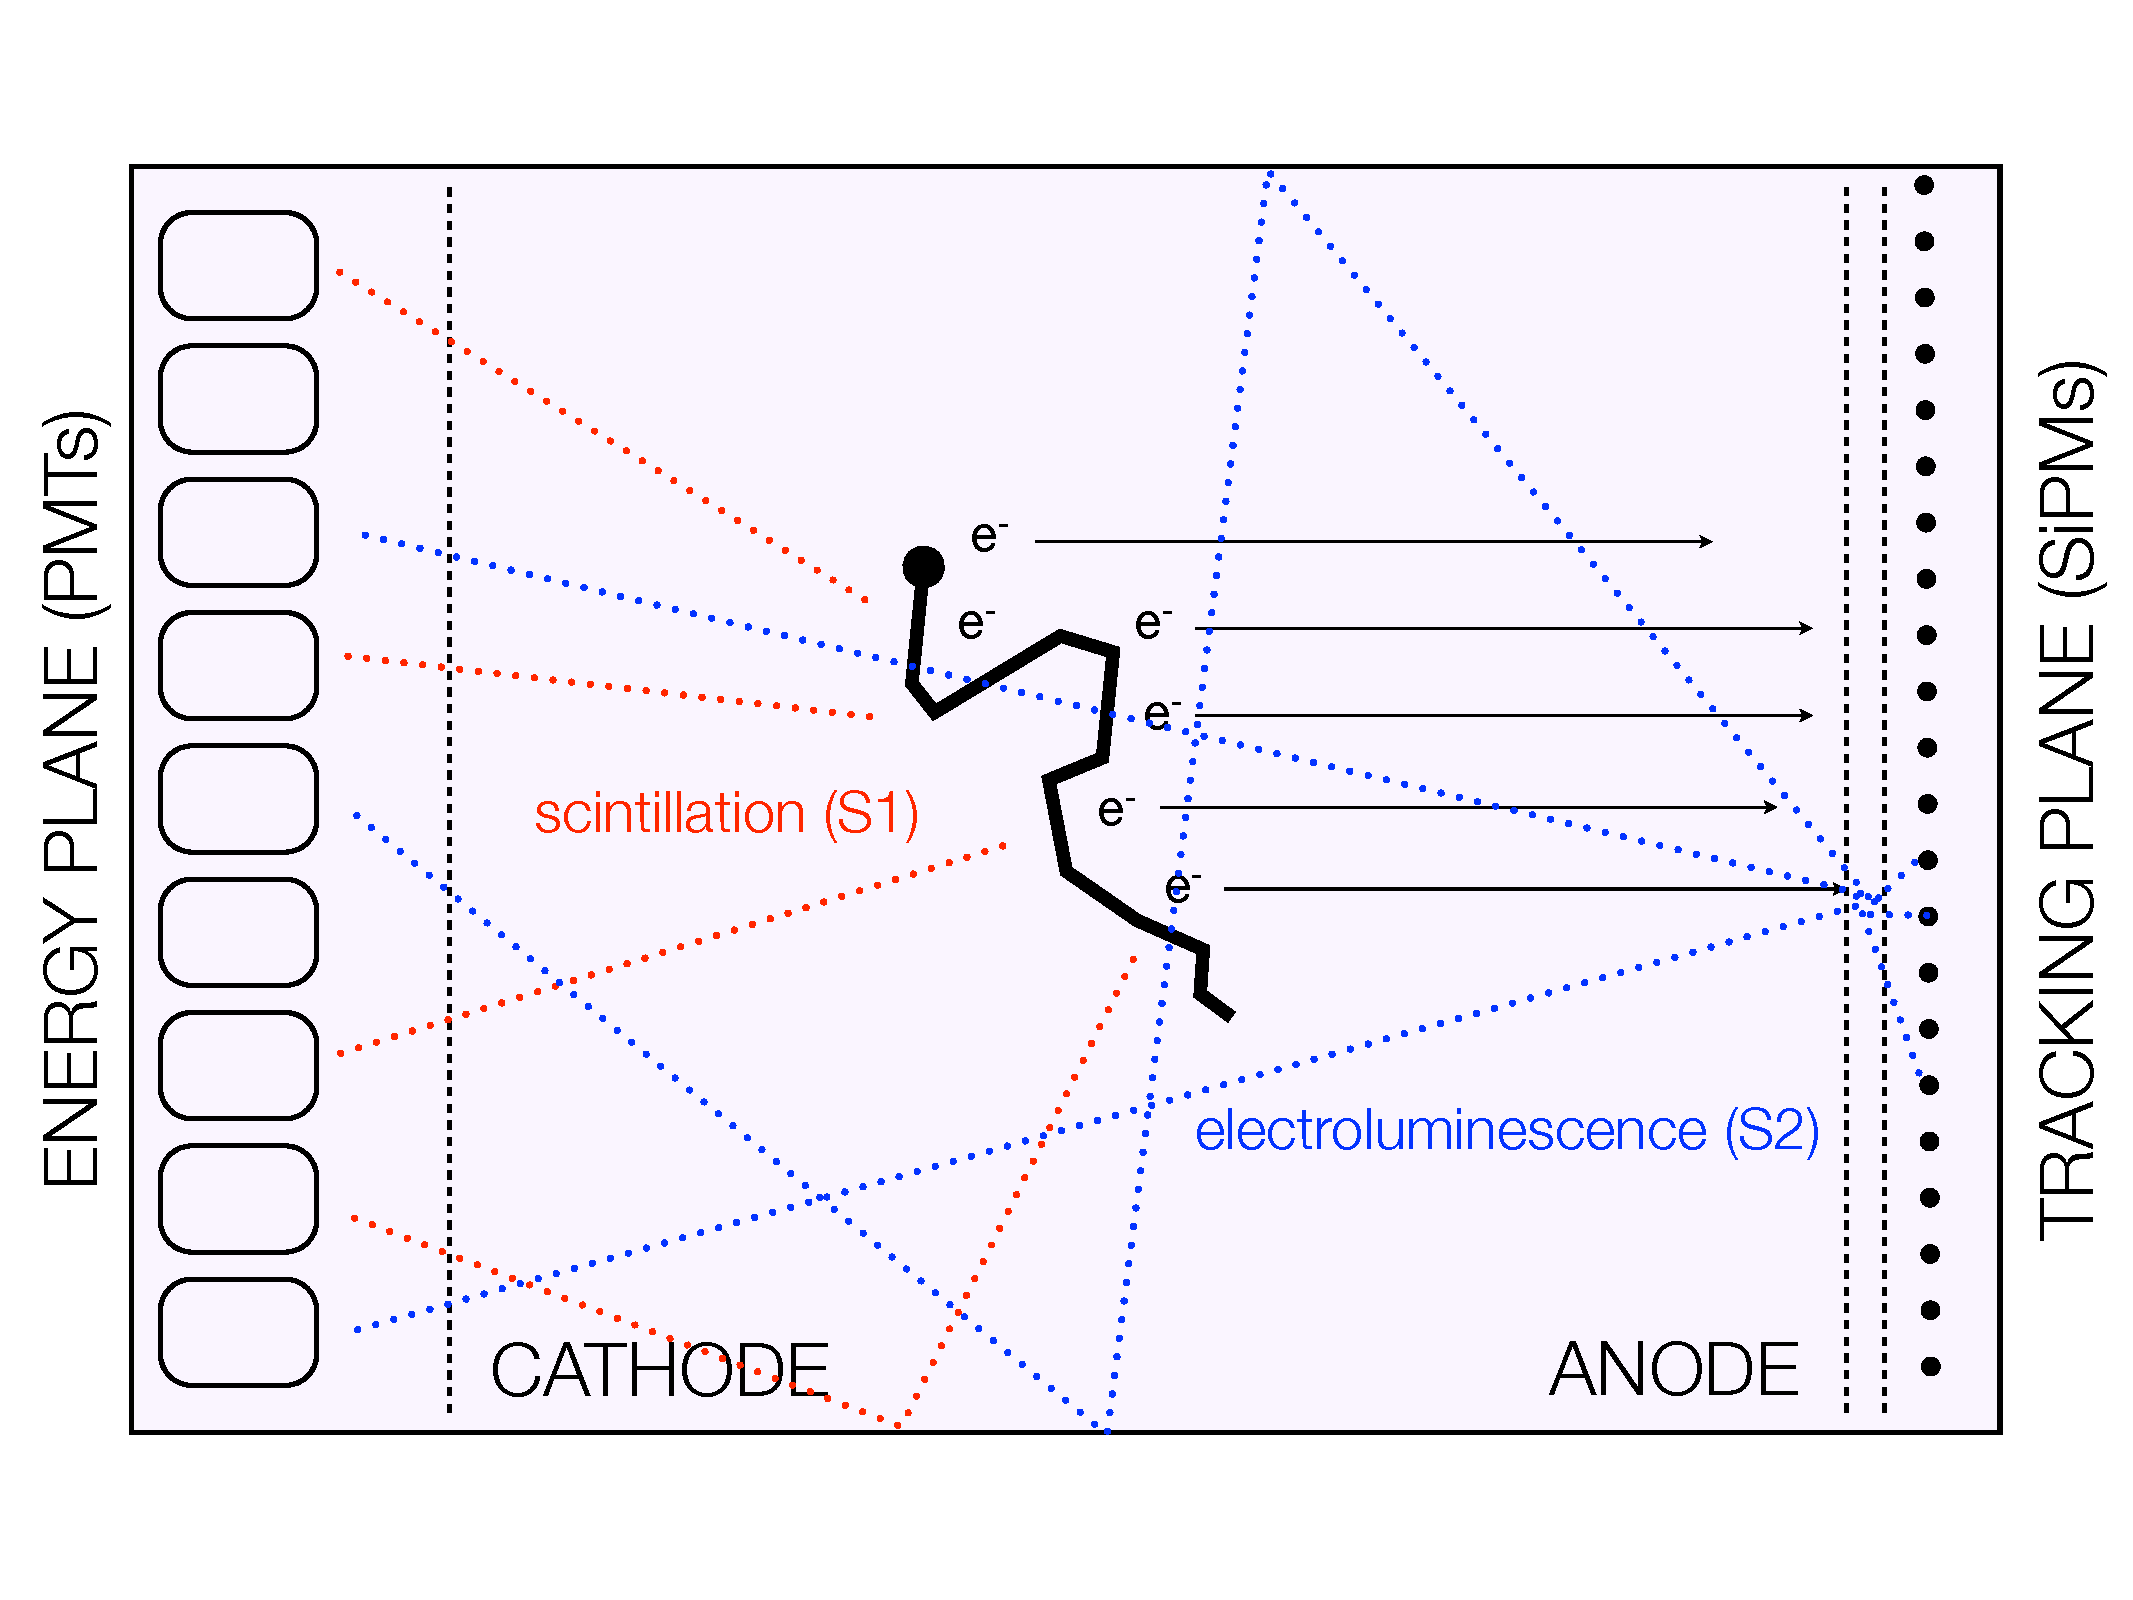
\includegraphics[width= 0.42\textwidth]{fig/nextEL.pdf}
	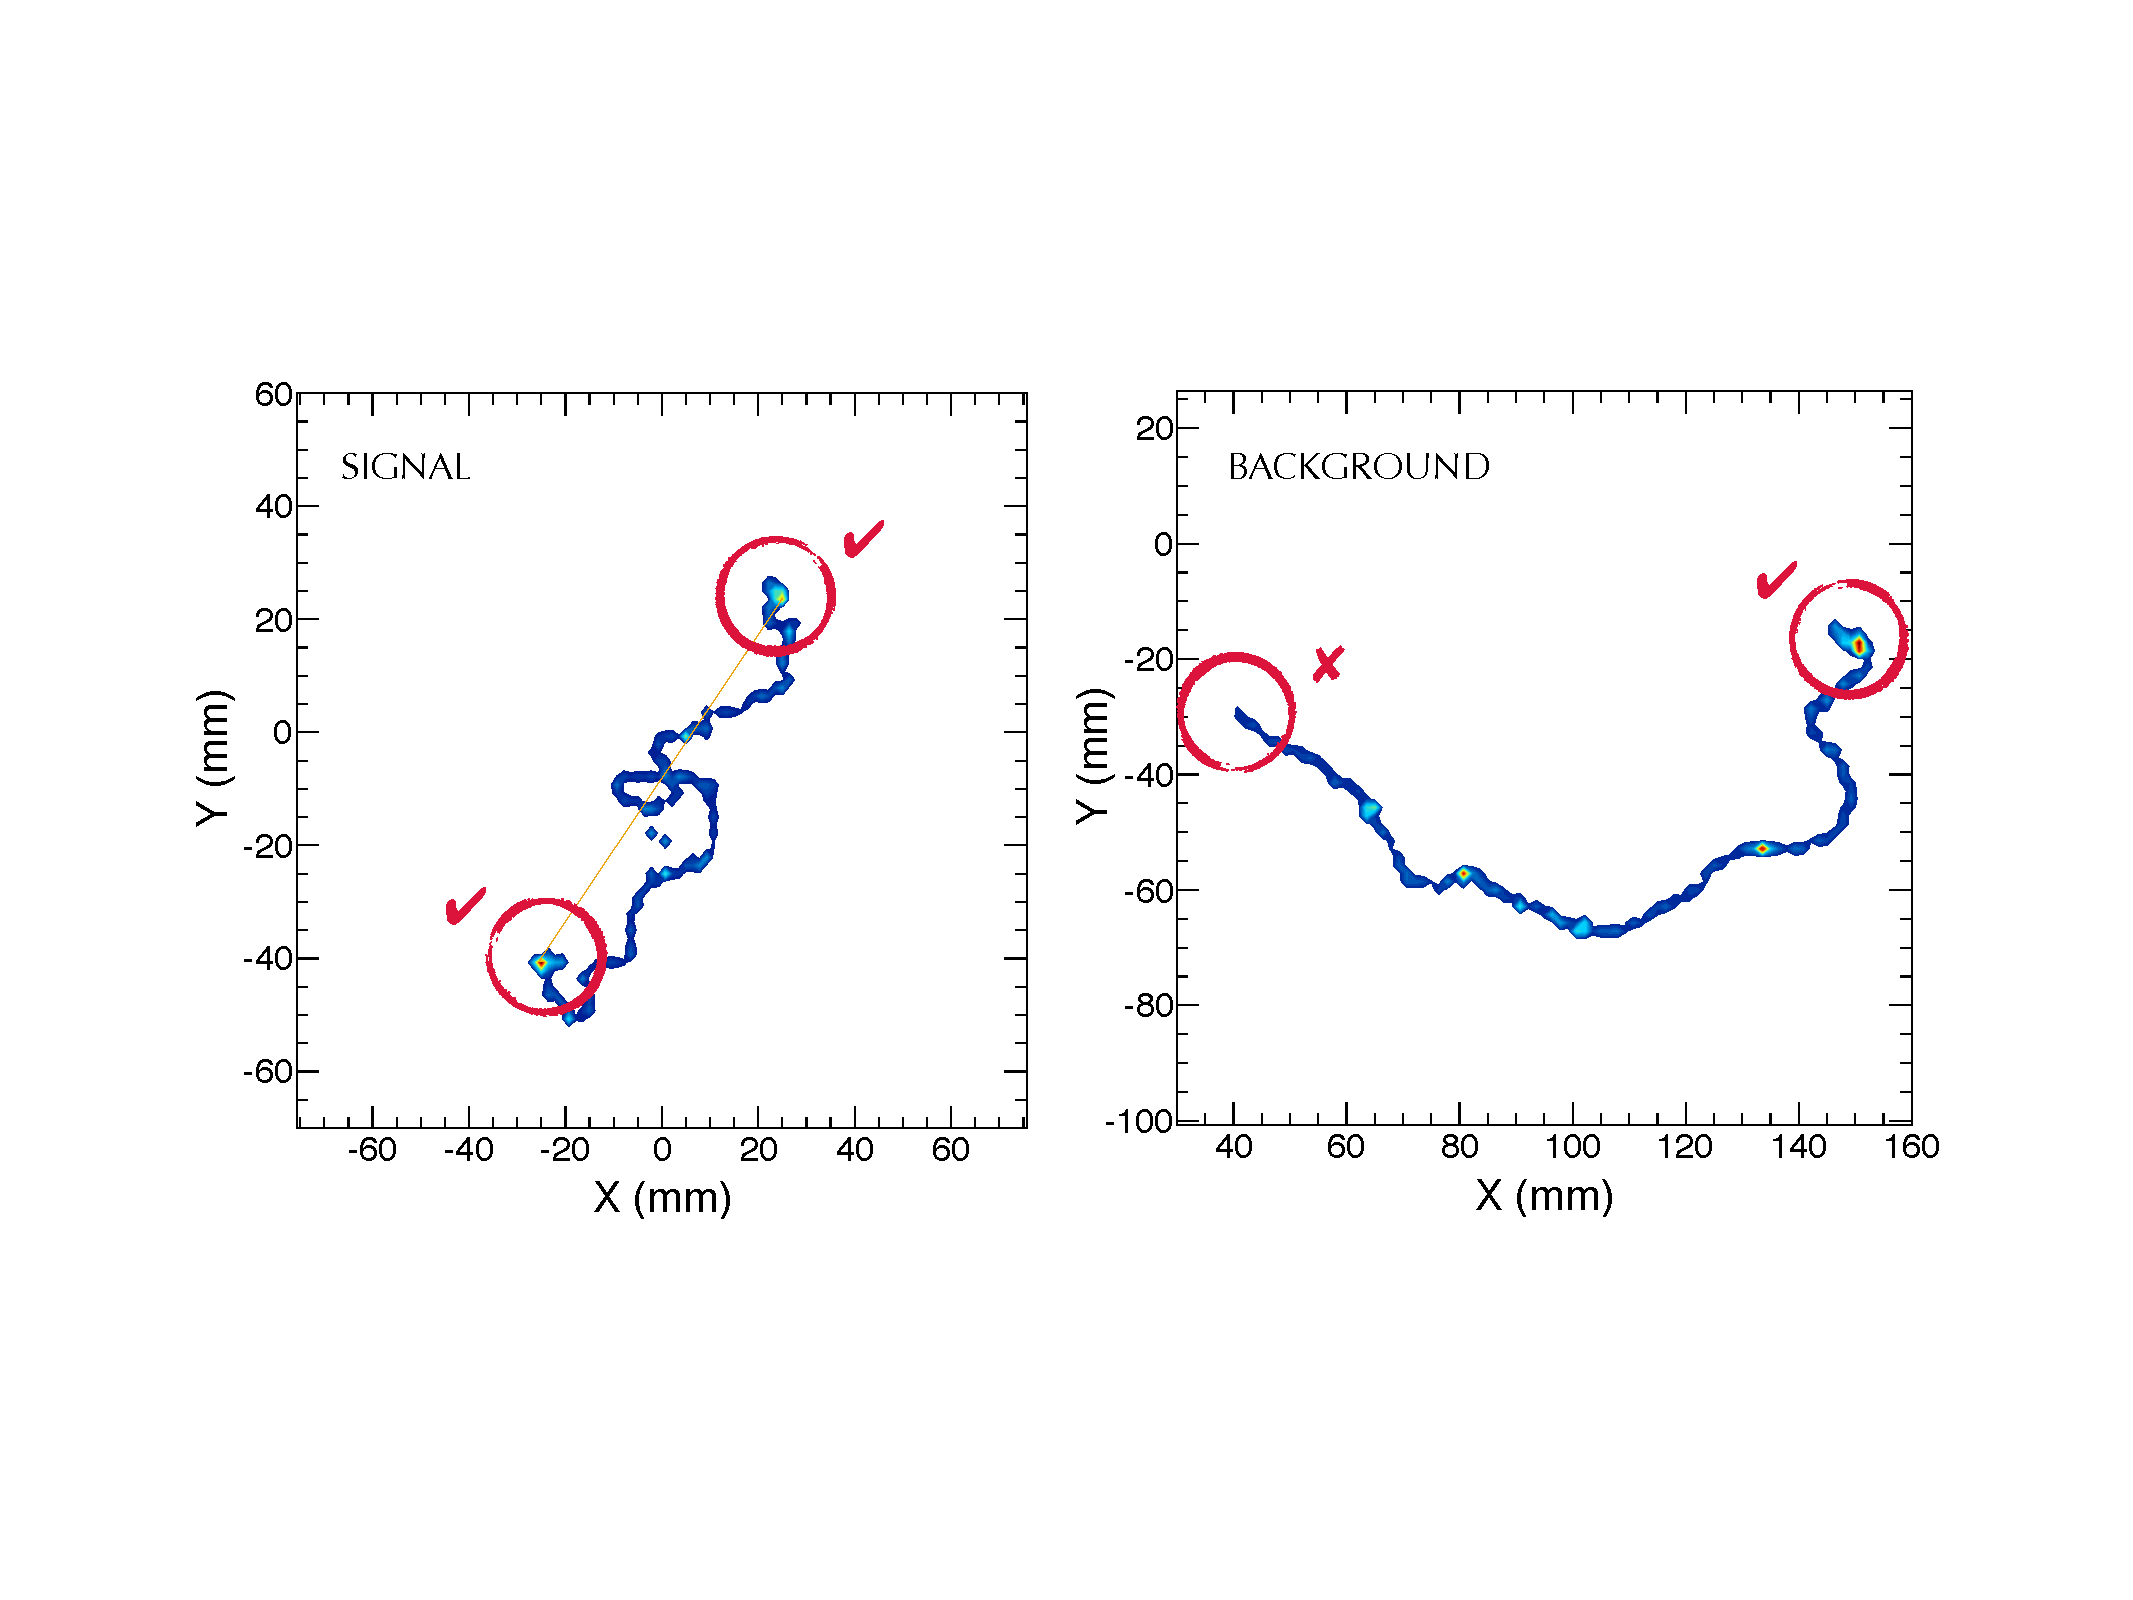
\includegraphics[width= 0.56\textwidth]{fig/TrackSignature.pdf}
	\caption{The NEXT concept. (Left, figure from \cite{Alvarez:2013gxa}) In an asymmetrical EL TPC, energetic electrons produce primary scintillation (S1) and ionization initially, and the ionization is drifted to the EL readout plane and amplified, producing additional scintillation photons (S2).  The energy (PMT) plane detects S1 (coordinate $z$) and S2 (energy), while the finer-resolution tracking (SiPM) plane measures S2 to deduce $(x,y)$ coordinates, resulting in a full 3D reconstruction of the track and its energy. (Right, figure from \cite{NEXT_sensitivity}) The anticipated topologies of signal and background events in a $0\nu\beta\beta$ search with high pressure xenon gas.} \label{fig.SS}
\end{figure}

In order to fully benefit from the potential of the topological signature, a sound procedure for track reconstruction and classification is essential. We have already shown ... but could do better (by a factor of 10?) with deep learning techniques.

\noindent\textbf{Deep Learning}\\

- also want to show how DNNs can be used in physics applications (IMPORTANT to note other potential benefits and give examples)
- diagram of proposed analysis construction chain

{\noindent\textbf{Section B: Methodology}}\\
Discuss use of Python (Keras, TF) and previous use of Caffe/DIGITS.  Discuss use of GPUs.  Develop plan for analysis and procedure for understanding DNNs.  Show what has already been done.\\

{\noindent\textbf{Section C: Resources (including project costs)}}\\

\bibliography{dnnext}

\end{document}